\documentclass[12pt]{article}
\usepackage[margin=1 in]{geometry}
\usepackage{graphicx}
\usepackage{float}
\usepackage{booktabs}
\usepackage{siunitx}
\usepackage{amsmath}


\title{Lab 7: Getting started with Operational Amplifier Circuits}
\author{Sean Balbale}
\date{October 25th, 2024}
\setlength{\parindent}{0in}

\begin{document}

\begin{titlepage}
	\begin{center}
		\vspace*{1in}

		\Huge
		\textbf{Lab 8}

		\LARGE
		Getting started with Analog to Digital Conversion and Sampling

		\vspace{3 in}

		\textbf{Student Name:} Sean Balbale
		\\ \textbf{Instructor:} Dr. Iman Salama
		\\ \textbf{Lab Partner Name:} Krish Gupta
		\\ \textbf{Date:} November 2, 2024

		\vfill


	\end{center}
\end{titlepage}

\newpage

\section{Introduction} 
The lab report introduces an exploration into Analog to Digital Conversion (ADC) 
and sampling techniques using National Instruments' (NI) USB-DAQ hardware and MATLAB 
software. The primary objective was to bridge continuous analog signals from the 
physical world into discrete digital signals that can be processed on a computer. 
Through practical exercises, foundational skills in configuring and utilizing the 
NI USB-6001 DAQ system for signal acquisition were developed, including manipulating 
data acquisition settings in MATLAB and analyzing the impacts of sampling rates and 
quantization errors on signal fidelity.
\newline

The lab emphasized understanding the trade-offs and limitations inherent in 
digitizing analog signals, such as quantization noise and sampling artifacts. The 
exercises demonstrated the effects of varying sampling rates and signal frequencies 
on digital audio quality. Additionally, signal 
degradation at lower sampling rates and the effects of quantization resolution on 
signal accuracy were explored.
\newline

Through experimentation with synthetic and real-world signals, this lab provided 
practical experience in digital signal processing concepts, preparing students for 
more advanced applications in biomedical engineering and other technical fields.
\newline

\section{Results}
% \begin{figure}[H]
% 	\centering
% 	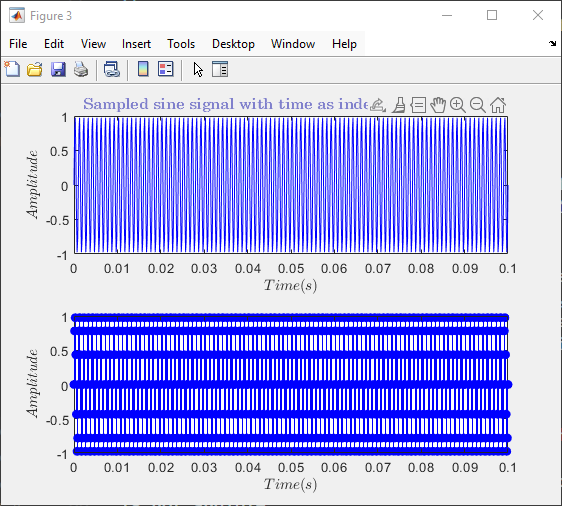
\includegraphics[width=0.3\textwidth]{fig 1f 7000.png}\hfill
% 	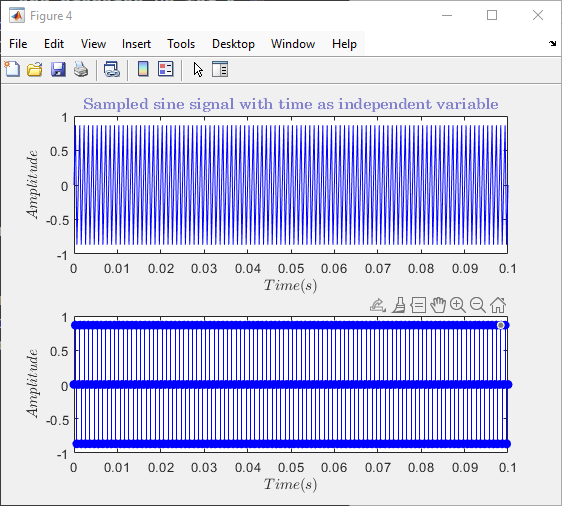
\includegraphics[width=0.3\textwidth]{fig 1f 3000.png}\hfill
% 	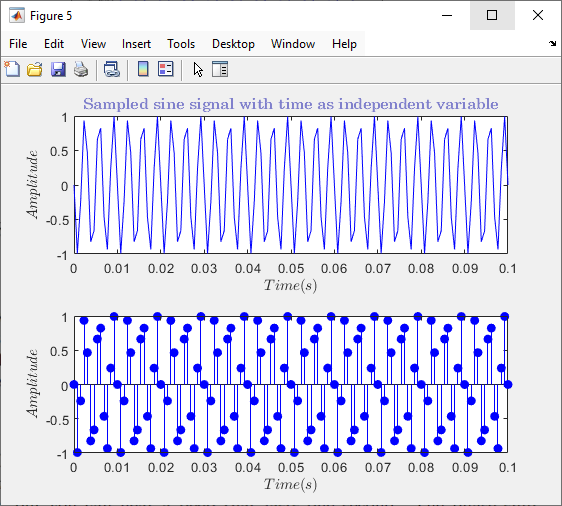
\includegraphics[width=0.3\textwidth]{fig 1f 1300.png}
% 	\caption{Sinusoidal with $f_s$ = 7 kHz, 3 kHz, and 1.3 kHz}
% 	\label{fig:fig3}
% % \end{figure}
\subsection{Basic Setup of the DAQ System}
In Part 1 of this lab, the DAQ system was set up to enable Analog to 
Digital Conversion. The NI USB-6001 DAQ device was connected to a 
computer, and its functionality was confirmed in MATLAB by executing 
the `daq.getDevices` command, which verified that the device was 
properly recognized. After establishing the connection, the DAQ 
configuration process continued with the addition of an analog input 
channel. This setup allowed the device to receive and process analog 
signals within a specific voltage range, adjusted for the parameters 
of the experiment.
\newline

The DAQ’s operating parameters were verified by checking the device’s 
voltage range, supported sampling rates, and channel capabilities, 
confirming that the device could handle the specified signal 
characteristics. MATLAB was used to set up the acquisition parameters, 
ensuring that the input signal could be accurately digitized for 
analysis. The DAQ was then prepared to acquire a test signal, with 
MATLAB configured to handle data acquisition through the appropriate 
commands and settings. This setup provided a foundation for capturing 
and analyzing continuous analog signals, converting them into a digital 
format suitable for the subsequent steps of the experiment.
\newline

\subsection{Inputting and Acquiring a Test Signal}
In Part 2, a test signal was input and acquired using the configured 
DAQ system. A sine wave with a frequency of 500 Hz and an amplitude of 
2V was generated by a function generator and connected to the DAQ. To 
allow simultaneous monitoring, the signal was also routed to an 
oscilloscope using a BNC to banana connector cable and alligator clips, 
enabling direct observation of the analog waveform. The DAQ was set to 
sample at a rate of 10,000 samples per second over a 0.01-second 
acquisition period, providing sufficient data to capture the 
characteristics of the input signal. 
MATLAB commands were employed to initiate the data acquisition and plot 
the resulting samples, displaying the digitized sine wave on a time scale.
\newline

\begin{figure}[H]
	\centering
	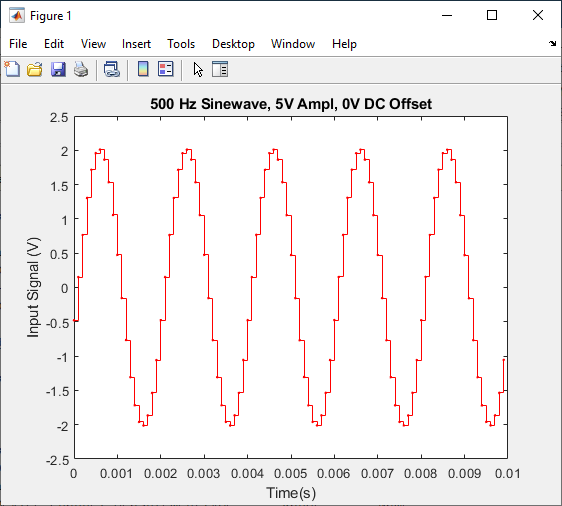
\includegraphics[width=0.5\textwidth]{fig 2.4.PNG}
	\caption{500 Hz Sinewave, 5V Amplitude, 0V DC Offset}
	\label{fig:fig1}
\end{figure}

The acquired signal was plotted, showing a clear sinusoidal shape that matched the properties of the input signal. This step demonstrated the DAQ’s ability to accurately capture and digitize an analog signal when properly configured with an adequate sampling rate. The successful acquisition and plotting of the signal validated the setup and provided a foundation for further experimentation with different signal types and configurations in later parts of the lab.
\newline

\subsection{Limitations of Digitization: Quantization Error}

\begin{figure}[H]
	\centering
	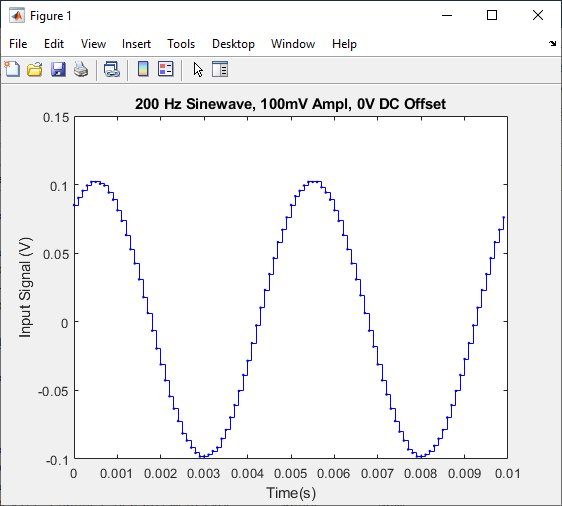
\includegraphics[width=0.5\textwidth]{fig 3.1.PNG}
	\caption{200 Hz Sinewave, 100mV Amplitude, Sampling Rate = 1500 Samples/Second}
	\label{fig:fig2}
\end{figure}

In Part 3, the lab explored the limitations of digitization, specifically 
focusing on quantization error, by analyzing two configurations of a 200 
Hz sine wave signal at low amplitudes. In Configuration 1 (Figure \ref{fig:fig2}), 
a sine wave with a 10 mV amplitude and 0V DC offset was sampled at a 
rate of 1500 samples per second. The resulting plot shows a stepped 
waveform with visible quantization effects, as the limited resolution 
of the DAQ's 14-bit ADC struggles to accurately represent the small 
amplitude changes of the signal. The digitized signal appears jagged, 
with clear discrete steps, indicating that the quantization levels do 
not adequately capture the subtle variations in the analog waveform. 
This quantization error becomes significant when working with 
low-amplitude signals, as the DAQ can only approximate the signal 
within the resolution of its 14-bit ADC.
\newline

\begin{figure}[H]
	\centering
	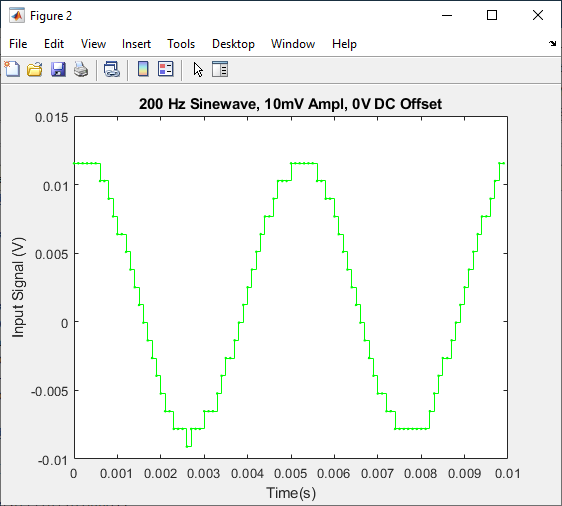
\includegraphics[width=0.5\textwidth]{fig 3.2.PNG}
	\caption{200 Hz Sinewave, 100mV Amplitude, Sampling Rate = 10000 Samples/Second}
	\label{fig:fig3}
\end{figure}

In Configuration 2 (Figure \ref{fig:fig3}), the sine wave amplitude was 
increased to 100 mV while maintaining the same frequency and DC offset, 
and the sampling rate was increased to 10,000 samples per second. The 
resulting waveform displays a much smoother sinusoidal shape with fewer 
visible steps, as the increased amplitude and higher sampling rate allow 
for a more accurate representation of the signal. The increased amplitude 
reduces the relative impact of quantization error, as the DAQ has more 
discrete levels to represent the larger signal. The higher sampling rate 
captures the waveform with greater detail, minimizing the stair-step 
effect seen in Configuration 1.
\newline

Comparing both configurations, it is clear that the amplitude of the 
input signal and the sampling rate significantly impact the quality 
of the digital representation. Lower amplitudes and sampling rates 
increase quantization artifacts, distorting the waveform and deviating 
from the original analog signal. This part of the lab illustrated the 
importance of selecting appropriate signal amplitudes and sampling rates 
to achieve a more accurate digital representation, particularly when 
working with signals at low amplitudes.
\newline

\subsection{Sampling Music or Speech}
In Part 4, the lab investigated the effects of different sampling rates on audio 
signal fidelity by digitizing a segment of the song "Happy Birthday." The audio 
signal was played from a phone and sampled using the DAQ device at three different 
rates: 20 kHz, 5 kHz, and 1 kHz. At the highest sampling rate of 20 kHz, the 
digitized audio maintained a clear and accurate representation of the original 
song, with minimal distortion and preserved tonal quality. This high sampling 
rate helped retain the nuances and details of the original music.
\newline

At a sampling rate of 5 kHz, the playback quality noticeably declined. Although 
the melody of "Happy Birthday" was still recognizable, the sound lacked clarity, 
and certain high-frequency details were lost, resulting in a muffled or slightly 
distorted sound. This drop in quality reflects the trade-off when reducing the 
sampling rate, as fewer samples per second capture less detail from the original 
signal.
\newline

At the lowest sampling rate of 1 kHz, the audio was heavily distorted, with 
significant artifacts. Much of the song’s tonal quality was lost, making it 
challenging to recognize the melody clearly. This very low sampling rate was 
insufficient for accurately capturing the range of frequencies present in the 
music, leading to severe degradation in sound quality. This exercise demonstrated 
how lower sampling rates can dramatically impact audio fidelity, especially in 
applications requiring accurate representation of complex signals like music. 
It highlighted the necessity of selecting an adequate sampling rate to ensure 
accurate digital reproduction, particularly in contexts where sound quality is 
critical.
\newline

\subsection{A/D Sampling Rate - Deeper Investigation}
In Part 5, the lab examined the relationship between sampling rate and the accurate 
digitization of higher-frequency signals. A 1 kHz sine wave was generated and sampled 
at multiple rates: 20,000 Hz, 10,000 Hz, 4,000 Hz, 2,500 Hz, 1,800 Hz, 1,600 Hz, 
1,400 Hz, and 1,200 Hz. At the higher sampling rates (20,000 Hz and 10,000 Hz), the 
digitized signal closely matched the original analog signal, with smooth, continuous 
sinusoidal waveforms observed upon playback. The high sampling rates provided ample 
data points to accurately capture the 1 kHz frequency, resulting in clear audio with 
minimal distortion.
\newline

As the sampling rate decreased to 4,000 Hz and 2,500 Hz, some minor distortion began 
to appear, but the 1 kHz frequency was still recognizable. However, at even lower 
rates, such as 1,800 Hz and 1,600 Hz, more significant distortion emerged, with 
visible artifacts and an increasingly “stepped” appearance in the waveform. By the 
time the sampling rate dropped to 1,400 Hz and 1,200 Hz, the audio was heavily 
distorted, with a pronounced loss in fidelity, making it difficult to identify the 
original 1 kHz tone. This degradation occurred because the lower sampling rates 
provided fewer points per cycle, resulting in an inaccurate representation of the 
original signal’s frequency and waveform.
\newline

This part of the lab highlighted the importance of selecting an appropriate sampling 
rate based on the frequency of the signal being captured. As demonstrated, sampling 
rates that are too low relative to the signal frequency result in noticeable 
distortion and can cause the signal to be misrepresented. Thus, for accurate 
digitization of signals, especially those with higher frequencies, a sufficiently 
high sampling rate is essential to ensure fidelity and avoid issues such as aliasing 
and waveform distortion.
\newline

\section{Discussion and Conclusion}
This lab provided a comprehensive exploration of Analog to Digital Conversion
(ADC) and the essential role of sampling rates and quantization in digital
signal representation. By configuring the NI USB-6001 DAQ system and observing
the impact of various sampling parameters on different signal types, the lab
highlighted the trade-offs inherent in digitizing analog signals. Parts 1 and 2
established a foundation for accurately capturing signals by ensuring correct
DAQ setup and input signal acquisition. Part 3 demonstrated how quantization
error, particularly in low-amplitude signals, can lead to signal distortion,
emphasizing the importance of choosing an appropriate amplitude and bit
resolution. In Part 4, the effect of sampling rate on audio fidelity was evident,
as lower rates introduced distortion and reduced clarity in the playback of
"Happy Birthday." Part 5 further reinforced that an adequate sampling rate is
essential for preserving the integrity of higher-frequency signals, as lower
sampling rates resulted in pronounced distortion and loss of signal detail.
\newline

Overall, this lab underscored key principles in digital signal processing, such
as the importance of sampling rate, quantization error, and bit resolution,
which are crucial considerations in applications like biomedical engineering,
audio processing, and communications. Understanding these concepts equips
students with the knowledge needed to optimize signal acquisition systems for
precise and accurate digital representations of real-world analog signals.
\section{References}
 [1] Dr. Iman Salama. “Lab 8 – Getting started with Analog to Digital Conversion and Sampling” Northeastern University. 2 November 2024.

\end{document}
